\documentclass[D:/studies/WinnerS/Erhebungen/IPhO1718/paper/problem_solving/main/TaylorFrancis/interactapasample]{subfiles}

%\usepackage{Sweave}

\begin{document}






\section{Results}


Since the motivational variables are self-reported measures and the cognitive variables likely tap similar cognitive abilities, it is necessary to investigate the correlations among the variables first in order to verify that no multi-collinearity is present. The correlations (Table \ref{correlation_table}) show values in the range between $-0.2-0.42$. However, most values are lower such that no multicollinearity is present. One pattern in the correlation matrix is that the cognitive variables correlate significantly amongst each other and the motivational variables correlate significantly amongst each other in positive directions. Social support shows almost no significant correlation with another variable. Interestingly, self-efficacy in physics is not correlated with cognitive variables, which is quiet counter-intuitive given the literature on self-efficacy (see: Bandura, 1997). Expectancy of success in the competition, however, is significantly correlated with the cognitive variables, possibly because it is more context-specific such that students can better judge their actual ability.

\begin{sidewaystable}
\caption{Correlations among measured variables.}
\label{correlation_table}
% latex table generated in R 3.4.3 by xtable 1.8-2 package
% Sun Jan 06 16:08:03 2019
\begin{tabular}{lcccccccccc}
  \toprule
Measure & 1 & 2 & 3 & 4 & 5 & 6 & 7 & 8 & 9 & 10 \\ 
  \midrule
1 Problem comprehension & - & .27** & .28*** & .10 & .18* & .18* & .01 & .01 & .40*** & .31*** \\ 
  2 Heuristic physics problem solving &  & - & .15 & .01 & .25** & -.09 & .05 & .09 & .32*** & .16 \\ 
  3 Cog. abilities &  &  & - & .04 & .18* & .01 & -.02 & -.20* & .16 & .13 \\ 
  4 Self-efficacy physics &  &  &  & - & .37*** & .28*** & .42*** & .12 & .12 & -.18* \\ 
  5 Expectancy physics competition &  &  &  &  & - & .21* & .34*** & .18* & .29*** & .04 \\ 
  6 Value physics competition &  &  &  &  &  & - & .28*** & .07 & .13 & -.07 \\ 
  7 Sense of belonging &  &  &  &  &  &  & - & .19* & .000 & -.01 \\ 
  8 Social support in physics &  &  &  &  &  &  &  & - & .01 & -.16 \\ 
  9 Highest round &  &  &  &  &  &  &  &  & - & .08 \\ 
  10 Age &  &  &  &  &  &  &  &  &  & - \\ 
   \bottomrule
\end{tabular}\end{sidewaystable}




In order to characterize successful particupants (RQ 1), generalized linear models that account for the ordinal metric of the dependent variable are utilized. Cognitive and motivational variables are included as predictors for highest qualified round (dependent variable). Achievement in round 1 in the physics Olympiad was omitted as a cognitive variable because of the high correlation with the other cognitive measures that were of more interest to us. Proportional odds models were used in order to predict success in the Physics Olympiad in a hierarchical regression procedure (Field, 2012). First, cognitive variables were included as predictors in the model because these predictors can be considered most important for characterizing successful students in the Physics Olympiad based on prior research. In a second step, cognitive variables and motivational variables were jointly entered in the model.

Generalized linear models, as any mathematical model, come with certain assumptions that need be tested prior to conducting the analysis. The modelling assumption of parallel slopes holds in our case, $\chi^2=2.2, p=.53$. 

The interesting parameters in the model are the effects (not the intercepts). The effects can be interpreted in accordance with the regression parameters in linear regression (B\"u{}rkner \& Vuorre, 2018). Table \ref{propOddModel} shows the results from the analysis. As can be expected, physics problem conceptualization and generic physics problem solving are significantly positively related with highest qualified round of the participants. The relationship holds when entering the motivational variables to the model. When all variables are included in the model, expectancy of success in the competition shows a significant positive relationship with highest qualified round as well. No other effects become significant and thus characterize successful students in this study. Physics problem conceptualization has the highest odds ratio, and thus a change in physics problem conceptualization of one standard deviation has the highest contribution to the likelihood of a student to reach a higher round. In order to graphically represent this relationship, Figure \ref{problem_concept_skills} depicts highest round over physics problem conceptualization skills.


\begin{table}
\caption{Proportional odds model for predicting highest qualified round in the physics Olympiad with various predictors.}
\label{propOddModel}
% latex table generated in R 3.4.3 by xtable 1.8-2 package
% Sun Jan 06 16:08:05 2019
\begin{tabular}{llcccc}
  \toprule
 & $\beta$ & $SE(\beta)$ & $z$ & $p$ & $OR$ \\ 
  \midrule
Phys. Prob. Conceptualization  & 0.71 & 0.19 & 3.65 & $<.001$ & 2.03 \\ 
  Heur. Phys. Prob. Sol.  & 0.51 & 0.19 & 2.68 & $<.01$ & 1.66 \\ 
  kft.c.imp.2  & 0.09 & 0.18 & 0.48 & $.63$ & 1.09 \\ 
   &  &  &  &  &  \\ 
  $R^2_{\text{adj}}$ & 0.24 &  &  &  &  \\ 
  \midrule Phys. Prob. Conceptualization & 0.7 & 0.21 & 3.28 & $<.001$ & 2.02 \\ 
  Heur. Phys. Prob. Sol. & 0.48 & 0.2 & 2.4 & $<.05$ & 1.61 \\ 
  Cog. abilities & 0.02 & 0.19 & 0.12 & $.90$ & 1.02 \\ 
  Self eff. & 0.1 & 0.22 & 0.44 & $.66$ & 1.1 \\ 
  Exp. phy. comp. & 0.54 & 0.22 & 2.45 & $<.01$ & 1.72 \\ 
  Val. phy. comp. & 0.14 & 0.2 & 0.71 & $.48$ & 1.15 \\ 
  Sen. of bel. & -0.32 & 0.21 & -1.52 & $.13$ & 0.73 \\ 
  Soc. sup. & -0.05 & 0.19 & -0.24 & $.81$ & 0.95 \\ 
  Age & -0.11 & 0.2 & -0.57 & $.57$ & 0.89 \\ 
    &  &  &  &  &  \\ 
  $R^2_{\text{adj}}$  & 0.3 &  &  &  &  \\ 
   \bottomrule
\end{tabular}\end{table}



\begin{figure}
\centering
% 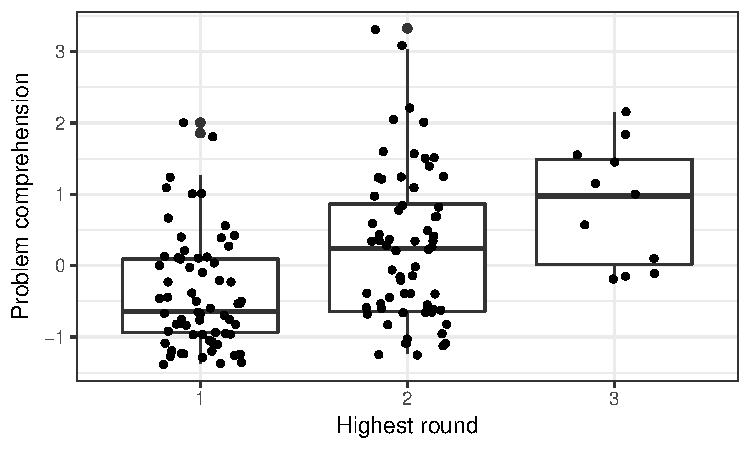
\includegraphics[width=.7\textwidth]{D:/studies/WinnerS/Erhebungen/IPhO1718/paper/problem_solving/results/ordinal_regression/img/boxplot}
% Created by tikzDevice version 0.11 on 2019-01-06 13:27:31
% !TEX encoding = UTF-8 Unicode
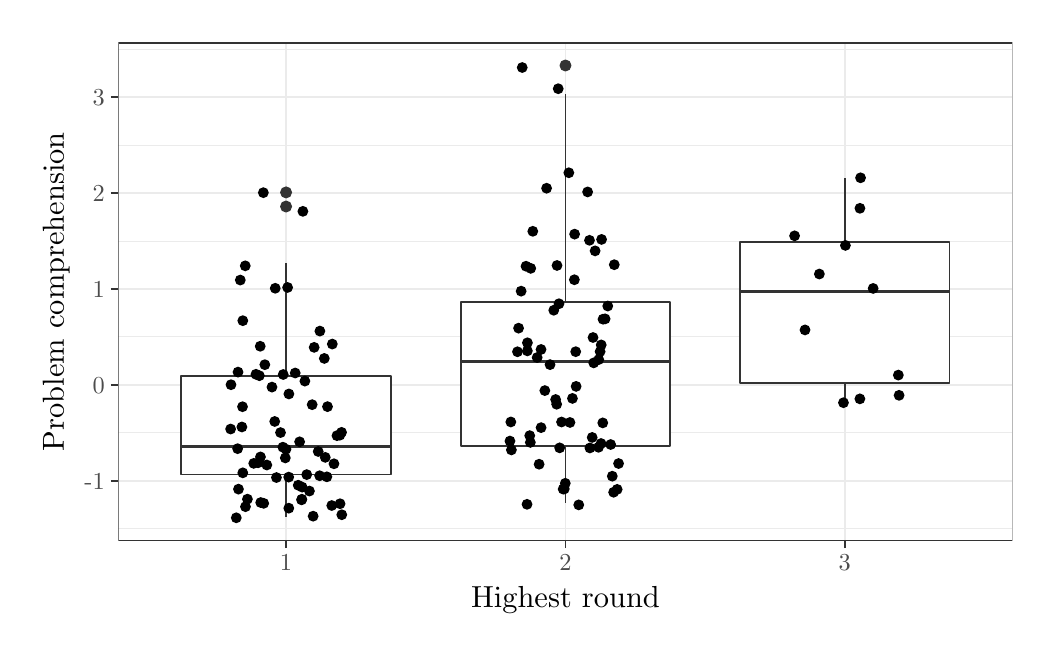
\begin{tikzpicture}[x=1pt,y=1pt]
\definecolor{fillColor}{RGB}{255,255,255}
\path[use as bounding box,fill=fillColor,fill opacity=0.00] (0,0) rectangle (361.35,216.81);
\begin{scope}
\path[clip] (  0.00,  0.00) rectangle (361.35,216.81);
\definecolor{drawColor}{RGB}{255,255,255}
\definecolor{fillColor}{RGB}{255,255,255}

\path[draw=drawColor,line width= 0.6pt,line join=round,line cap=round,fill=fillColor] (  0.00,  0.00) rectangle (361.35,216.81);
\end{scope}
\begin{scope}
\path[clip] ( 32.80, 31.53) rectangle (355.85,211.31);
\definecolor{fillColor}{RGB}{255,255,255}

\path[fill=fillColor] ( 32.80, 31.53) rectangle (355.85,211.31);
\definecolor{drawColor}{gray}{0.92}

\path[draw=drawColor,line width= 0.3pt,line join=round] ( 32.80, 35.77) --
	(355.85, 35.77);

\path[draw=drawColor,line width= 0.3pt,line join=round] ( 32.80, 70.42) --
	(355.85, 70.42);

\path[draw=drawColor,line width= 0.3pt,line join=round] ( 32.80,105.08) --
	(355.85,105.08);

\path[draw=drawColor,line width= 0.3pt,line join=round] ( 32.80,139.73) --
	(355.85,139.73);

\path[draw=drawColor,line width= 0.3pt,line join=round] ( 32.80,174.39) --
	(355.85,174.39);

\path[draw=drawColor,line width= 0.3pt,line join=round] ( 32.80,209.05) --
	(355.85,209.05);

\path[draw=drawColor,line width= 0.6pt,line join=round] ( 32.80, 53.10) --
	(355.85, 53.10);

\path[draw=drawColor,line width= 0.6pt,line join=round] ( 32.80, 87.75) --
	(355.85, 87.75);

\path[draw=drawColor,line width= 0.6pt,line join=round] ( 32.80,122.41) --
	(355.85,122.41);

\path[draw=drawColor,line width= 0.6pt,line join=round] ( 32.80,157.06) --
	(355.85,157.06);

\path[draw=drawColor,line width= 0.6pt,line join=round] ( 32.80,191.72) --
	(355.85,191.72);

\path[draw=drawColor,line width= 0.6pt,line join=round] ( 93.37, 31.53) --
	( 93.37,211.31);

\path[draw=drawColor,line width= 0.6pt,line join=round] (194.33, 31.53) --
	(194.33,211.31);

\path[draw=drawColor,line width= 0.6pt,line join=round] (295.28, 31.53) --
	(295.28,211.31);
\definecolor{drawColor}{gray}{0.20}
\definecolor{fillColor}{gray}{0.20}

\path[draw=drawColor,line width= 0.4pt,line join=round,line cap=round,fill=fillColor] ( 93.37,152.18) circle (  1.96);

\path[draw=drawColor,line width= 0.4pt,line join=round,line cap=round,fill=fillColor] ( 93.37,157.28) circle (  1.96);

\path[draw=drawColor,line width= 0.6pt,line join=round] ( 93.37, 91.04) -- ( 93.37,131.80);

\path[draw=drawColor,line width= 0.6pt,line join=round] ( 93.37, 55.37) -- ( 93.37, 40.09);
\definecolor{fillColor}{RGB}{255,255,255}

\path[draw=drawColor,line width= 0.6pt,line join=round,line cap=round,fill=fillColor] ( 55.52, 91.04) --
	( 55.52, 55.37) --
	(131.23, 55.37) --
	(131.23, 91.04) --
	( 55.52, 91.04) --
	cycle;

\path[draw=drawColor,line width= 1.1pt,line join=round] ( 55.52, 65.56) -- (131.23, 65.56);
\definecolor{fillColor}{gray}{0.20}

\path[draw=drawColor,line width= 0.4pt,line join=round,line cap=round,fill=fillColor] (194.33,203.14) circle (  1.96);

\path[draw=drawColor,line width= 0.6pt,line join=round] (194.33,117.79) -- (194.33,192.95);

\path[draw=drawColor,line width= 0.6pt,line join=round] (194.33, 65.56) -- (194.33, 45.18);
\definecolor{fillColor}{RGB}{255,255,255}

\path[draw=drawColor,line width= 0.6pt,line join=round,line cap=round,fill=fillColor] (156.47,117.79) --
	(156.47, 65.56) --
	(232.18, 65.56) --
	(232.18,117.79) --
	(156.47,117.79) --
	cycle;

\path[draw=drawColor,line width= 1.1pt,line join=round] (156.47, 96.13) -- (232.18, 96.13);

\path[draw=drawColor,line width= 0.6pt,line join=round] (295.28,139.45) -- (295.28,162.38);

\path[draw=drawColor,line width= 0.6pt,line join=round] (295.28, 88.49) -- (295.28, 80.85);

\path[draw=drawColor,line width= 0.6pt,line join=round,line cap=round,fill=fillColor] (257.42,139.45) --
	(257.42, 88.49) --
	(333.14, 88.49) --
	(333.14,139.45) --
	(257.42,139.45) --
	cycle;

\path[draw=drawColor,line width= 1.1pt,line join=round] (257.42,121.61) -- (333.14,121.61);
\definecolor{fillColor}{RGB}{0,0,0}

\path[fill=fillColor] (195.95, 74.15) circle (  1.96);

\path[fill=fillColor] (184.10, 97.61) circle (  1.96);

\path[fill=fillColor] ( 75.87, 64.68) circle (  1.96);

\path[fill=fillColor] (280.89,107.59) circle (  1.96);

\path[fill=fillColor] (300.96,162.56) circle (  1.96);

\path[fill=fillColor] (100.84, 55.31) circle (  1.96);

\path[fill=fillColor] ( 98.97, 46.19) circle (  1.96);

\path[fill=fillColor] (192.92, 74.32) circle (  1.96);

\path[fill=fillColor] ( 85.70, 95.03) circle (  1.96);

\path[fill=fillColor] (210.66, 66.18) circle (  1.96);

\path[fill=fillColor] (174.79, 64.24) circle (  1.96);

\path[fill=fillColor] (190.77, 82.45) circle (  1.96);

\path[fill=fillColor] ( 77.74,110.93) circle (  1.96);

\path[fill=fillColor] ( 83.28, 59.59) circle (  1.96);

\path[fill=fillColor] ( 89.89, 54.25) circle (  1.96);

\path[fill=fillColor] (208.65,111.58) circle (  1.96);

\path[fill=fillColor] (207.81, 74.00) circle (  1.96);

\path[fill=fillColor] (108.11, 54.51) circle (  1.96);

\path[fill=fillColor] (203.99, 68.74) circle (  1.96);

\path[fill=fillColor] ( 83.72, 91.05) circle (  1.96);

\path[fill=fillColor] (207.25,102.17) circle (  1.96);

\path[fill=fillColor] (206.27, 65.18) circle (  1.96);

\path[fill=fillColor] ( 97.76, 51.47) circle (  1.96);

\path[fill=fillColor] (294.78, 81.29) circle (  1.96);

\path[fill=fillColor] ( 81.69, 59.37) circle (  1.96);

\path[fill=fillColor] (192.23, 64.98) circle (  1.96);

\path[fill=fillColor] (204.29,104.85) circle (  1.96);

\path[fill=fillColor] ( 92.22, 65.22) circle (  1.96);

\path[fill=fillColor] ( 84.03,101.69) circle (  1.96);

\path[fill=fillColor] ( 77.73, 55.95) circle (  1.96);

\path[fill=fillColor] ( 99.45,150.44) circle (  1.96);

\path[fill=fillColor] (197.64,142.20) circle (  1.96);

\path[fill=fillColor] ( 79.40, 46.44) circle (  1.96);

\path[fill=fillColor] (207.38,140.29) circle (  1.96);

\path[fill=fillColor] ( 78.62,130.75) circle (  1.96);

\path[fill=fillColor] (186.88, 85.67) circle (  1.96);

\path[fill=fillColor] (211.73, 48.94) circle (  1.96);

\path[fill=fillColor] (197.55,125.72) circle (  1.96);

\path[fill=fillColor] ( 75.38, 39.70) circle (  1.96);

\path[fill=fillColor] (202.34,157.45) circle (  1.96);

\path[fill=fillColor] (203.16, 64.94) circle (  1.96);

\path[fill=fillColor] ( 96.67, 92.02) circle (  1.96);

\path[fill=fillColor] ( 94.33, 54.41) circle (  1.96);

\path[fill=fillColor] ( 73.47, 87.79) circle (  1.96);

\path[fill=fillColor] ( 93.10, 61.34) circle (  1.96);

\path[fill=fillColor] ( 78.70, 43.72) circle (  1.96);

\path[fill=fillColor] ( 77.41, 72.52) circle (  1.96);

\path[fill=fillColor] ( 92.34, 91.48) circle (  1.96);

\path[fill=fillColor] (104.98, 63.66) circle (  1.96);

\path[fill=fillColor] ( 85.16,157.19) circle (  1.96);

\path[fill=fillColor] (110.08,102.48) circle (  1.96);

\path[fill=fillColor] (277.12,141.59) circle (  1.96);

\path[fill=fillColor] (198.18, 87.19) circle (  1.96);

\path[fill=fillColor] (196.85, 82.84) circle (  1.96);

\path[fill=fillColor] ( 91.36, 70.50) circle (  1.96);

\path[fill=fillColor] (181.78,129.84) circle (  1.96);

\path[fill=fillColor] (195.55,164.38) circle (  1.96);

\path[fill=fillColor] ( 93.93,122.93) circle (  1.96);

\path[fill=fillColor] (180.08,130.61) circle (  1.96);

\path[fill=fillColor] (180.58,102.94) circle (  1.96);

\path[fill=fillColor] ( 94.36, 43.18) circle (  1.96);

\path[fill=fillColor] (174.27, 67.43) circle (  1.96);

\path[fill=fillColor] (300.72, 82.68) circle (  1.96);

\path[fill=fillColor] (110.68, 59.22) circle (  1.96);

\path[fill=fillColor] ( 99.08, 46.41) circle (  1.96);

\path[fill=fillColor] (193.50, 50.08) circle (  1.96);

\path[fill=fillColor] (191.28,130.88) circle (  1.96);

\path[fill=fillColor] (111.76, 69.38) circle (  1.96);

\path[fill=fillColor] ( 89.27, 74.51) circle (  1.96);

\path[fill=fillColor] (198.03, 99.73) circle (  1.96);

\path[fill=fillColor] (204.54, 95.69) circle (  1.96);

\path[fill=fillColor] ( 73.34, 71.78) circle (  1.96);

\path[fill=fillColor] (199.13, 44.37) circle (  1.96);

\path[fill=fillColor] ( 76.83,125.61) circle (  1.96);

\path[fill=fillColor] (113.50, 40.81) circle (  1.96);

\path[fill=fillColor] (101.81, 49.37) circle (  1.96);

\path[fill=fillColor] (206.85, 99.77) circle (  1.96);

\path[fill=fillColor] (206.35, 96.88) circle (  1.96);

\path[fill=fillColor] ( 82.49, 91.56) circle (  1.96);

\path[fill=fillColor] ( 76.17, 50.06) circle (  1.96);

\path[fill=fillColor] (112.81, 69.56) circle (  1.96);

\path[fill=fillColor] (107.19, 97.29) circle (  1.96);

\path[fill=fillColor] (191.15, 80.73) circle (  1.96);

\path[fill=fillColor] ( 93.35, 64.48) circle (  1.96);

\path[fill=fillColor] ( 77.63, 79.84) circle (  1.96);

\path[fill=fillColor] ( 76.01, 92.35) circle (  1.96);

\path[fill=fillColor] (193.90, 50.14) circle (  1.96);

\path[fill=fillColor] (113.42, 70.58) circle (  1.96);

\path[fill=fillColor] (174.59, 74.33) circle (  1.96);

\path[fill=fillColor] (191.71,194.75) circle (  1.96);

\path[fill=fillColor] ( 84.21, 45.22) circle (  1.96);

\path[fill=fillColor] (184.81, 59.06) circle (  1.96);

\path[fill=fillColor] ( 86.42, 58.78) circle (  1.96);

\path[fill=fillColor] (203.01,139.97) circle (  1.96);

\path[fill=fillColor] (300.73,151.54) circle (  1.96);

\path[fill=fillColor] ( 98.27, 67.16) circle (  1.96);

\path[fill=fillColor] ( 88.28, 86.93) circle (  1.96);

\path[fill=fillColor] ( 89.46,122.64) circle (  1.96);

\path[fill=fillColor] (182.53,143.23) circle (  1.96);

\path[fill=fillColor] (295.49,138.13) circle (  1.96);

\path[fill=fillColor] (181.64, 66.95) circle (  1.96);

\path[fill=fillColor] ( 94.39, 84.45) circle (  1.96);

\path[fill=fillColor] (181.42, 69.39) circle (  1.96);

\path[fill=fillColor] (103.15, 40.29) circle (  1.96);

\path[fill=fillColor] (176.99, 99.70) circle (  1.96);

\path[fill=fillColor] (305.51,122.58) circle (  1.96);

\path[fill=fillColor] ( 99.17, 50.80) circle (  1.96);

\path[fill=fillColor] (213.52, 59.31) circle (  1.96);

\path[fill=fillColor] ( 84.12, 61.70) circle (  1.96);

\path[fill=fillColor] (180.56,100.02) circle (  1.96);

\path[fill=fillColor] (286.07,127.79) circle (  1.96);

\path[fill=fillColor] (314.61, 91.27) circle (  1.96);

\path[fill=fillColor] (112.88, 44.78) circle (  1.96);

\path[fill=fillColor] (102.80, 80.58) circle (  1.96);

\path[fill=fillColor] (211.25, 54.74) circle (  1.96);

\path[fill=fillColor] (191.99,117.05) circle (  1.96);

\path[fill=fillColor] (103.52,101.29) circle (  1.96);

\path[fill=fillColor] (188.76, 95.05) circle (  1.96);

\path[fill=fillColor] (209.61,116.22) circle (  1.96);

\path[fill=fillColor] (185.50,100.53) circle (  1.96);

\path[fill=fillColor] (211.97,131.16) circle (  1.96);

\path[fill=fillColor] (187.51,158.79) circle (  1.96);

\path[fill=fillColor] (207.90,111.47) circle (  1.96);

\path[fill=fillColor] (213.01, 49.97) circle (  1.96);

\path[fill=fillColor] (194.27, 52.16) circle (  1.96);

\path[fill=fillColor] (185.52, 72.28) circle (  1.96);

\path[fill=fillColor] (190.10,114.70) circle (  1.96);

\path[fill=fillColor] (177.39,108.23) circle (  1.96);

\path[fill=fillColor] ( 85.29, 44.93) circle (  1.96);

\path[fill=fillColor] (105.59,107.17) circle (  1.96);

\path[fill=fillColor] (105.51, 54.90) circle (  1.96);

\path[fill=fillColor] (109.88, 44.14) circle (  1.96);

\path[fill=fillColor] (108.34, 79.87) circle (  1.96);

\path[fill=fillColor] (207.19, 66.54) circle (  1.96);

\path[fill=fillColor] (178.31,121.60) circle (  1.96);

\path[fill=fillColor] (205.04,136.15) circle (  1.96);

\path[fill=fillColor] (178.71,202.41) circle (  1.96);

\path[fill=fillColor] (107.53, 61.54) circle (  1.96);

\path[fill=fillColor] (100.17, 89.10) circle (  1.96);

\path[fill=fillColor] (180.44, 44.58) circle (  1.96);

\path[fill=fillColor] (314.88, 83.96) circle (  1.96);

\path[draw=drawColor,line width= 0.6pt,line join=round,line cap=round] ( 32.80, 31.53) rectangle (355.85,211.31);
\end{scope}
\begin{scope}
\path[clip] (  0.00,  0.00) rectangle (361.35,216.81);
\definecolor{drawColor}{gray}{0.30}

\node[text=drawColor,anchor=base east,inner sep=0pt, outer sep=0pt, scale=  0.88] at ( 27.85, 50.06) {-1};

\node[text=drawColor,anchor=base east,inner sep=0pt, outer sep=0pt, scale=  0.88] at ( 27.85, 84.72) {0};

\node[text=drawColor,anchor=base east,inner sep=0pt, outer sep=0pt, scale=  0.88] at ( 27.85,119.38) {1};

\node[text=drawColor,anchor=base east,inner sep=0pt, outer sep=0pt, scale=  0.88] at ( 27.85,154.03) {2};

\node[text=drawColor,anchor=base east,inner sep=0pt, outer sep=0pt, scale=  0.88] at ( 27.85,188.69) {3};
\end{scope}
\begin{scope}
\path[clip] (  0.00,  0.00) rectangle (361.35,216.81);
\definecolor{drawColor}{gray}{0.20}

\path[draw=drawColor,line width= 0.6pt,line join=round] ( 30.05, 53.10) --
	( 32.80, 53.10);

\path[draw=drawColor,line width= 0.6pt,line join=round] ( 30.05, 87.75) --
	( 32.80, 87.75);

\path[draw=drawColor,line width= 0.6pt,line join=round] ( 30.05,122.41) --
	( 32.80,122.41);

\path[draw=drawColor,line width= 0.6pt,line join=round] ( 30.05,157.06) --
	( 32.80,157.06);

\path[draw=drawColor,line width= 0.6pt,line join=round] ( 30.05,191.72) --
	( 32.80,191.72);
\end{scope}
\begin{scope}
\path[clip] (  0.00,  0.00) rectangle (361.35,216.81);
\definecolor{drawColor}{gray}{0.20}

\path[draw=drawColor,line width= 0.6pt,line join=round] ( 93.37, 28.78) --
	( 93.37, 31.53);

\path[draw=drawColor,line width= 0.6pt,line join=round] (194.33, 28.78) --
	(194.33, 31.53);

\path[draw=drawColor,line width= 0.6pt,line join=round] (295.28, 28.78) --
	(295.28, 31.53);
\end{scope}
\begin{scope}
\path[clip] (  0.00,  0.00) rectangle (361.35,216.81);
\definecolor{drawColor}{gray}{0.30}

\node[text=drawColor,anchor=base,inner sep=0pt, outer sep=0pt, scale=  0.88] at ( 93.37, 20.52) {1};

\node[text=drawColor,anchor=base,inner sep=0pt, outer sep=0pt, scale=  0.88] at (194.33, 20.52) {2};

\node[text=drawColor,anchor=base,inner sep=0pt, outer sep=0pt, scale=  0.88] at (295.28, 20.52) {3};
\end{scope}
\begin{scope}
\path[clip] (  0.00,  0.00) rectangle (361.35,216.81);
\definecolor{drawColor}{RGB}{0,0,0}

\node[text=drawColor,anchor=base,inner sep=0pt, outer sep=0pt, scale=  1.10] at (194.33,  7.44) {Highest round};
\end{scope}
\begin{scope}
\path[clip] (  0.00,  0.00) rectangle (361.35,216.81);
\definecolor{drawColor}{RGB}{0,0,0}

\node[text=drawColor,rotate= 90.00,anchor=base,inner sep=0pt, outer sep=0pt, scale=  1.10] at ( 13.08,121.42) {Problem comprehension};
\end{scope}
\end{tikzpicture}

\caption{Problem conceptualization scores over highest achieved round of participant.}
\label{problem_concept_skills}
\end{figure}

\end{document}
